\documentclass{article}
\usepackage[utf8]{inputenc}
\usepackage{natbib}
\usepackage{graphicx}
\usepackage{float}
\usepackage{chngcntr}
\counterwithin{figure}{section}

\title{SVG to PES CAD Tool}
\author{Austyn Larkin}
\date{2018-11-14}

\pdfpagewidth 8.5in
\pdfpageheight 11in

\begin{document}
\maketitle
\section{Intro}
Home sewing machines are becoming so advanced that some now include the ability to embroider designs onto cloth. Pre-made designs can be selected from the machine's memory or new designs can be downloaded to the machine using a USB flash drive. If a user wants to make their own design, they need to download embroidery software to their desktop computer. However, most embroidery software is very expensive and is not affordable for hobbyists or home users. In this paper, we propose a new CAD tool to convert a common vector shape format (.SVG) to the embroidery format used by machines such as the Brother® SE600 (.PES).

\section{Background}

\subsection{The SVG File Format}

\cite{SVGFormat} describes the SVG file format in detail. An SVG is a scalable vector graphic. It utilizes XML to allow for the description of two-dimensional vector graphics. Although the SVG format can be used to describe a number of common shapes, the only aspect of interest will be the paths. Paths within the SVG format allow for the description of arbitrary vector shapes. These paths are made up of quadratic and cubic Bézier curves. Each test SVG design is exclusively made up of one or more paths. The svgPathTools library \cite{svgpathtools} will be used to read and perform intersections on the test SVG paths. The SVG file format was chosen as it is a common and widely supported. Free software such as Inkscape [4] can export user designs to the SVG format. An example of an SVG can be seen in Figure \ref{appleExample}.

\begin{figure}[H]
    \centering
    \includegraphics[width=2in]{SVGExample}
    \caption{An SVG that contains three separate paths.}
    \label{appleExample}
\end{figure}

\subsection{The PES File Format}

Although the PES file format is proprietary, major parts of the format have been reverse engineered \cite{PESFormat}. The file format is primarily used by Brother and Bernina International machines. The format can be divided by its three major parts: the header, the PES section, and the PEC section.

The header starts with the "magic number" that specifies that the file is a PES file. This is simply the four characters that spell "\#PES". Four more characters follow after which determine the version number.

The PES section contains higher level stitch information. This includes individual stitches but also later versions of the PES format allow common shapes to be specified. This portion of the file was largely ignored as it's used by desktop embroidery software and not by the embroidery machine.

The PEC section contains the actual commands and data that the embroidery machine uses to embroider a design. The major aspects are listed as follows: The PEC header contains the thread colors that should be used when embroidering the design. For PES version 1, thread colors are represented as integer indices in a known list of thread colors specific to the format. Each thread color index is listed in the PEC header and will show up on the embroidery machine in the order they should be loaded. The command list is made up of four different command types: short stitch, long stitch, jump stitch, and color change. Short stitches are two bytes. Each byte specifies how far to move in the X and Y directions before making the next stitch. A long stitch is similar, except each axis takes up two bytes. This is to allow for extra movement distance and some bit flags. If the 12th bit is set in a long stitch command, the command is a jump stitch command. This tells the sewing machine to make a loose stitch that can be cut away later. These stitches are necessary so the machine can jump between discontinuous stitch regions in the design. The last command is a color change command. It tells the machine to stop so the user can swap out the thread color before continuing.

\section{Software Description}

The software was written as a command line tool in Python. A number of arguments can be passed to the program. This allows the user to set parameters such as parallel stitch distance and max stitch length. The program takes an SVG file as an input and produces a PES file as an output. The software works by intersecting each path in the SVG shape with an array of parallel lines. From these lines, the software figures out where stitches should go. It then takes these stitches and makes them continuous. It finishes by encoding the stitches in the PES format and saving the file to disk. To accomplish this, a number of Python libraries were used \cite{svgpathtools} \cite{numpy} \cite{pyEmbroidery}. A detailed example of this process is described in chronological order by Figures \ref{p-1} through \ref{p8}.

\begin{figure}[H]
    \centering
    \includegraphics[width=3in]{p-1}
    \caption{The SVG file that will be used for the example. This shape was chosen as it has many concave regions.}
    \label{p-1}
\end{figure}

\begin{figure}[H]
    \centering
    \includegraphics[width=3in]{p0}
    \caption{The loaded SVG file. The dark blue lines are the outline of the shape. The light blue outline is the bounding box of the shape. The light green line is the "path line" that determines the angle of the intersection lines that are created. The slope of this line can be changed with the "-l" command line argument and will control the slope of the stitches formed.}
    \label{p0}
\end{figure}

\begin{figure}[H]
    \centering
    \includegraphics[width=3in]{p1}
    \caption{The shape with the intersection lines (the gray lines) overlaid on top. An intersection is performed between the shape and each of the intersection lines. The points of each intersection operation are saved and used in the next step.}
    \label{p1}
\end{figure}

\begin{figure}[H]
    \centering
    \includegraphics[width=3in]{p2}
    \caption{The results of the intersections. Each intersection point is marked by a pink dot. Intersections should occur in pairs, since any line that enters the object has to leave the object. These intersection points are used to form the base stitches.}
    \label{p2}
\end{figure}

\begin{figure}[H]
    \centering
    \includegraphics[width=3in]{p3}
    \caption{The shape with the base stitches (red lines) overlaid on top. By themselves, these stitches are too long for the machine to perform. Performing these stitches would significantly stretch the cloth and distort the shape. Additionally, this shape cannot be stitched continuously. The machine will have to stitch as much as it can in one region and then jump to the next region with a jump stitch.}
    \label{p3}
\end{figure}

\begin{figure}[H]
    \centering
    \includegraphics[width=3in]{p4}
    \caption{The different stitch regions automatically determined by the software. Each region is marked by a different color. Color variation within each region shows separate stitches.}
    \label{p4}
\end{figure}

\begin{figure}[H]
    \centering
    \includegraphics[width=3in]{p5}
    \caption{Large stitches have now been broken up into smaller stitches. This is shown by the now greater color variation within each parallel stitch. Parallel stitches have also been connected "vertically" at the ends to make each region continuous.}
    \label{p5}
\end{figure}

\begin{figure}[H]
    \centering
    \includegraphics[width=3in]{p6}
    \caption{The software has added jump stitches between the different regions (marked by the white lines).}
    \label{p6}
\end{figure}

\begin{figure}[H]
    \centering
    \includegraphics[width=3in]{p7}
    \caption{"Outline" stitches have been added that traverse the entire boundary of the shape. Despite being created at the end of the process, these stitches are prepended to the stitch list so they will be performed first.}
    \label{p7}
\end{figure}

\begin{figure}[H]
    \centering
    \includegraphics[width=3in]{p8}
    \caption{The results of stitching the finished PES file on a Brother SE600 sewing machine. The jump stitches are visible on the shape. These are necessary so the machine can reach every region on the shape and are manually cut away after the machine has finished. This is to be expected when embroidering.}
    \label{p8}
\end{figure}

\section{Experimental Setup}

A total of 14 benchmarks were performed to test the software. The first set contained four benchmarks which tested the software's ability to handle a variety of path shapes, path curves, and files containing multiple paths. The SVGs in Figures \ref{appleSVG}, \ref{dropletSVG}, \ref{treeSVG}, and \ref{zigzagSVG} were run through the software to generate PES files. The settings used for the software were 1.5 (0.15mm) for the thread width and 20 (2mm) for the max stitch distance.

\begin{figure}[H]
    \centering
    \includegraphics[width=3in]{appleSVG}
    \caption{A very simple apple SVG. This benchmark tests the software's ability to handle multiple paths.}
    \label{appleSVG}
\end{figure}

\begin{figure}[H]
    \centering
    \includegraphics[width=3in]{dropletSVG}
    \caption{A blue droplet SVG. This is to test the software's ability to handle curves.}
    \label{dropletSVG}
\end{figure}

\begin{figure}[H]
    \centering
    \includegraphics[width=3in]{treeSVG}
    \caption{A tree SVG. This tests the software's ability to handle multiple paths in addition to curves.}
    \label{treeSVG}
\end{figure}

\begin{figure}[H]
    \centering
    \includegraphics[width=3in]{zigzagSVG}
    \caption{An SVG of a very odd shape. The concavity of this shape make it an excellent benchmark for testing the software's ability to form stitch regions and jump stitches.}
    \label{zigzagSVG}
\end{figure}

The next two sets of benchmarks were used to determine the effect of the software's settings on embroidery results. In hindsight, these tests also helped determine reasonable settings for embroidering. Each of the following tests used the droplet SVG in Figure \ref{dropletSVG} as the standard shape.

The second set of benchmarks varied the max stitch length. The max stitch length controls how long a single substitch is allowed to be. Four tests were performed using 0.5mm, 1.0mm, 1.5mm, and 2.0mm as the max stitch length. The thread width was held constant at 0.25mm.

The third set of benchmarks varied the thread width. The thread width controls the distance between the parallel lines that are intersected with the shape. Consequently, this also controls how close parallel stitches are to one another. Decreasing the thread width should increase the density of fill stitches. Four tests were performed with 0.15mm, 0.25mm, 0.35mm, and 0.45mm as the thread width.

The fourth set of benchmarks demonstrated the two different fill stitch settings for the software: continuous and zigzag. These two tests each used 0.25mm as the thread width and 2mm as the max stitch length.

For each of the tests described above, the generated PES files were embroidered as follows: A Brothher SE600 embroidery machine was set up in embroidery mode. A piece of white flannel was cut to fit the included embroidery hoop. An identically sized piece of Pellon Wash-N-Gone Stabilizer was cut and placed behind the piece of flannel. (Stabilizer is necessary to prevent cloth from stretching while embroidering and generally improves embroidery quality.) Each PES file was then embroidered, swapping thread colors and re-threading the needle as necessary. If the thread broke while embroidering, the machine was moved back 10 to 3 stitches, the needle was re-threaded, and then the machine was resumed.

\section{Results}

\subsection{First Set of Benchmarks}

The results of the first set of benchmarks are shown in Figures \ref{apple}, \ref{droplet}, \ref{tree}, \ref{zigzag}. Three different types of defects can be observed in the results. 

The first type of defect is the misalignment of the fill stitches with the outline stitches. This will be referred to as "fill stitch misalignment". Fill stitch misalignment is noticeable in the upper right corners of the apple, droplet, and tree. This phenomenon is possibly related to the order the stitches are performed in. 

The second type of defect will be referred to as "clumping". Clumping can be seen where stitches enter a thin segment, particularly at the bottom left corners of the apple's leaf and the tree's trunk.

The third defect will simply be referred to as "gaps". Gaps are seen any time the fill stitches fail to "fill" the shape fully. Multiple, tiny gaps are visible in the apple. This is most likely due to how the fill stitches are calculated.

\begin{figure}[H]
    \centering
    \includegraphics[width=3in]{apple}
    \caption{The embroidered apple.}
    \label{apple}
\end{figure}

\begin{figure}[H]
    \centering
    \includegraphics[width=3in]{droplet}
    \caption{The embroidered droplet.}
    \label{droplet}
\end{figure}

\begin{figure}[H]
    \centering
    \includegraphics[width=3in]{tree}
    \caption{The embroidered tree.}
    \label{tree}
\end{figure}

\begin{figure}[H]
    \centering
    \includegraphics[width=3in]{zigzag}
    \caption{The embroidered zigzag shape. The jump stitches have not been cut away and are still visible in the photo.}
    \label{zigzag}
\end{figure}

\subsection{Second Set of Benchmarks}

The results of the second set of benchmarks can be seen in Figures \ref{4_5w}, \ref{3_5w}, \ref{2_5w}, and \ref{1_5w}. As expected, the stitches get progressively denser as the thread width is reduced. Fill stitch misalignment can be seen in every benchmark. The 0.45mm thread width benchmark exhibited very little or no fill stitch misalignment. Of the four benchmarks, the 0.15mm thread width benchmark in Figure \ref{1_5w} reveals the least white cloth behind it. The 0.15mm thread width benchmark also shows the worst fill stitch alignment.

\begin{figure}[H]
    \centering
    \includegraphics[width=4.7in]{4_5w}
    \caption{The droplet embroidered with a thread width of 4.5 (0.45mm).}
    \label{4_5w}
\end{figure}

\begin{figure}[H]
    \centering
    \includegraphics[width=4.7in]{3_5w}
    \caption{The droplet embroidered with a thread width of 3.5 (0.35mm).}
    \label{3_5w}
\end{figure}

\begin{figure}[H]
    \centering
    \includegraphics[width=4.7in]{2_5w}
    \caption{The droplet embroidered with a thread width of 2.5 (0.25mm).}
    \label{2_5w}
\end{figure}

\begin{figure}[H]
    \centering
    \includegraphics[width=4.7in]{1_5w}
    \caption{The droplet embroidered with a thread width of 1.5 (0.15mm).}
    \label{1_5w}
\end{figure}

\subsection{Third Set of Benchmarks}

The third set of benchmarks can be seen in Figures \ref{20m}, \ref{15m}, \ref{10m}, and \ref{5m}. Of these four benchmarks, the 2mm max stitch length benchmark had the least fill stitch misalignment. Fill stitch misalignment got progressively worse as the max stitch length was decreased.

\begin{figure}[H]
    \centering
    \includegraphics[width=4.7in]{20m}
    \caption{The benchmark with the max stitch distance set to 20 (2mm).}
    \label{20m}
\end{figure}

\begin{figure}[H]
    \centering
    \includegraphics[width=4.7in]{15m}
    \caption{The benchmark with the max stitch distance set to 15 (1.5mm).}
    \label{15m}
\end{figure}

\begin{figure}[H]
    \centering
    \includegraphics[width=4.7in]{10m}
    \caption{The benchmark with the max stitch distance set to 10 (1.0mm).}
    \label{10m}
\end{figure}

\begin{figure}[H]
    \centering
    \includegraphics[width=4.7in]{5m}
    \caption{The benchmark with the max stitch distance set to 5 (0.5mm).}
    \label{5m}
\end{figure}

\subsection{Fourth Set of Benchmarks}

The fourth set of benchmarks can be seen in Figures \ref{StitchModeClosest_w2_5_d20}, \ref{StitchModeZigzag_w2_5_d20}. The benchmark that used the zigzag method generally had a very dense, consistent fill. It did exhibit bad fill stitch alignment, though. The benchmark that used the continuous method was most consistent. Because of the way the continuous method works, the fill stitches weren't as dense. This could be fixed by decreasing the thread width in future embroideries.

\begin{figure}[H]
    \centering
    \includegraphics[width=4.7in]{StitchModeClosest_w2_5_d20}
    \caption{}
    \label{StitchModeClosest_w2_5_d20}
\end{figure}

\begin{figure}[H]
    \centering
    \includegraphics[width=4.7in]{StitchModeZigzag_w2_5_d20}
    \caption{}
    \label{StitchModeZigzag_w2_5_d20}
\end{figure}

\section{Conclusion}

In this paper, conversion software between the SVG file format and the PES format was discussed and tested with 14 benchmarks. The paper detailed the methodologies in using loaded SVG shapes to generate stitches that could be performed by an embroidery machine. The 14 benchmarks were split up into four different groups. The first group of benchmarks tested the software's ability to handle different shapes and multiple paths within the same file. The second set of benchmarks tested the droplet shape with varying thread width. The third set of benchmarks tested the droplet shape with varying max stitch length. The fourth set of benchmarks demonstrated the "zigzag" and "continuous" methods of stitching available in the software. The first group of benchmarks showed that the software could handle various path shapes, curved paths, and multi-path SVG files. The second set of benchmarks showed that a thread width of 0.45mm gave the least fill stitch misalignment while 0.15mm gave the densest fill. The third set of benchmarks showed that a max stitch length of 2mm produced the most consistent results. From the benchmarks, reasonable default settings were determined for the software. These settings are 1.5 thread width, 20 max stitch length, and the "continuous" stitch method.

\section{Future Work}

Several areas for future work are apparent. The first is to reduce or minimize the errors observed in the benchmarks. This includes reducing or eliminating fill stitch misalignment, reducing clumping, and reducing gaps in finished, embroidered designs. Additional work should include testing general methods and techniques available for embroidering to rule out user error. Finally, while command line tools are useful to those who are familiar with Bash, they're not very user-friendly. Efforts to produce a user interface for the software would greatly improve accessibility within the sewing community.

\bibliographystyle{plain}
\bibliography{references}
\end{document}